% !TeX document-id = {2870843d-1baa-4f6a-bd0a-a5c796104a32}
% !BIB TS-program = biber
% !TeX encoding = UTF-8
% TU Delft beamer template

\documentclass[aspectratio=43]{beamer}
\usepackage[english]{babel}
\usepackage{csquotes}
\usepackage{calc}
\usepackage[absolute,overlay]{textpos}
\usepackage{graphicx}
\usepackage{subfig}
\usepackage{mathtools}
\usepackage{amsfonts}
\usepackage{amsthm}
\usepackage{comment}
\usepackage{siunitx}
\usepackage{MnSymbol,wasysym}
\usepackage{array}
\usepackage{qrcode}

\setbeamertemplate{navigation symbols}{} % remove navigation symbols
\mode<presentation>{\usetheme[verticalbar=false]{tud}}

% BIB SETTINGS
\usepackage[
    backend=biber,
    giveninits=true,
    maxnames=30,
    maxcitenames=20,
    uniquename=init,
    url=false,
    style=authoryear,
]{biblatex}
\addbibresource{bibfile.bib}
\setlength\bibitemsep{0.3cm} % space between entries in the reference list
\renewcommand{\bibfont}{\normalfont\scriptsize}
\setbeamerfont{footnote}{size=\tiny}
\renewcommand{\cite}[1]{\footnote<.->[frame]{\fullcite{#1}}}
\setlength{\TPHorizModule}{\paperwidth}
\setlength{\TPVertModule}{\paperheight}

\newcommand{\absimage}[4][0.5,0.5]{%
	\begin{textblock}{#3}%width
		[#1]% alignment anchor within image (centered by default)
		(#2)% position on the page (origin is top left)
		\includegraphics[width=#3\paperwidth]{#4}%
\end{textblock}}

\newcommand{\mininomen}[2][1]{{\let\thefootnote\relax%
	\footnotetext{\begin{tabular}{*{#1}{@{\!}>{\centering\arraybackslash}p{1em}@{\;}p{\textwidth/#1-2em}}}%
	#2\end{tabular}}}}


% to solve spurious empty pages before a frame containing footnotes
\setbeamertemplate{footnote}{%
  \makebox[1em][l]{\insertfootnotemark}%
  \begin{minipage}{\dimexpr\linewidth-1em}
    \usebeamerfont{footnote}\insertfootnotetext
  \end{minipage}\vskip 0pt}


\title[]{StarDataCapture: A Novel method for Analyzing Images in Space}
\institute[]{Institute for Computing in Research, Santa Fe}
\author{Rune Shultz}
%\date{}

\begin{document}
\section{Introduction}
{
\setbeamertemplate{footline}{\usebeamertemplate*{minimal footline}}
\frame{\titlepage}
}

\begin{frame}\Huge
  \frametitle{StarDataCapture}
  \begin{itemize}
      \centering
      \item Background
      \item Limitations
      \item Improvement?
  \end{itemize}
\end{frame}

\begin{frame}{How Does it Work?}
  \centering
  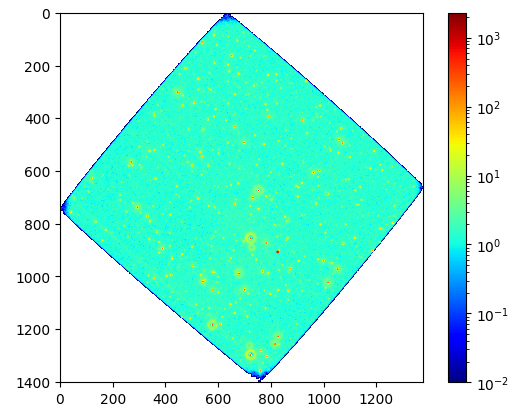
\includegraphics[scale = .5]{starexample.png}
\end{frame}

\begin{frame}{How Does it Work?}
  \centering
  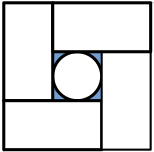
\includegraphics[scale = .75]{circleshape.png}
\end{frame}

\begin{frame}{Numerical Results}
  \centering
  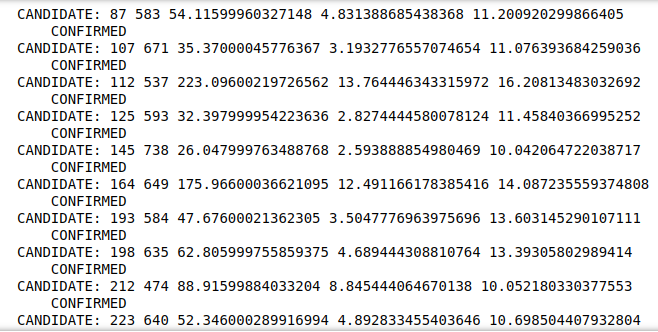
\includegraphics[scale = .5]{starnum1.png}
\end{frame}

\begin{frame}{Numerical Results}
  \centering
  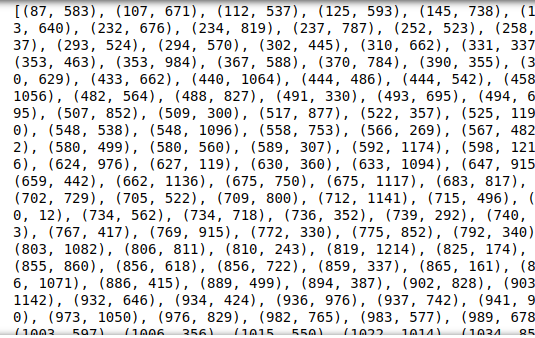
\includegraphics[scale = .5]{starcoords.png}
\end{frame}
\begin{frame}{Image Results}
  \centering
  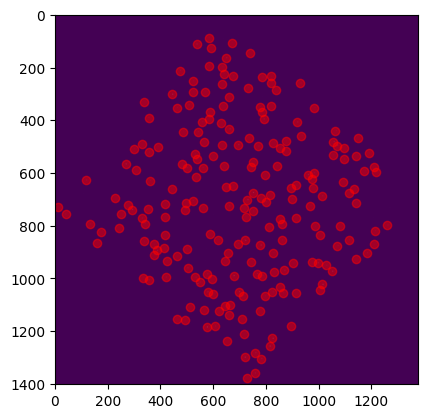
\includegraphics[scale = .75]{finalresults.png}
\end{frame}

\end{document}

